% \pagebreak[4]
% \hspace*{1cm}
% \pagebreak[4]
% \hspace*{1cm}
% \pagebreak[4]
%\usepackage[round,colon,authoryear]{natbib}

\chapter{Detecting rho-independent terminators in genomic sequence with covariance models}
\label{sec:chapterPingpong}
\ifpdf
    \graphicspath{{Chapter4/Chapter4Figs/EPS/}{Chapter4/Chapter4Figs/}}
\fi

\textit{Portions of this chapter are based on the previously published article ``RNIE: genome-wide prediction of bacterial intrinsic terminators'' \parencite{Gardner2011a}. This work is the result of collaboration with Paul P. Gardner (Wellcome Trust Sanger Institute/University of Canterbury). }

\section{Introduction}

Bacteria are thought to utilize two major systems for transcriptional termination: rho-dependent termination, and rho-independent or intrinsic termination \parencite{Peters2011}. Rho-dependent termination relies on a protein cofactor, Rho, a homohexameric ring protein that threads its way along the newly synthesized RNA molecule before causing RNA polymerase (RNAP\nomenclature[Z]{RNAP}{RNA polymerase}) to dissociate at poorly defined pause sites. Intrinsic termination on the other hand, depends primarily on the biophysical characteristics of the sequence being transcribed, and the discovery of these intrinsic terminators in genomic sequence is the subject of this chapter. This chapter will serve largely as background and motivation for the next, in which I develop computational methods for identifying and characterizing transcriptional termination motifs across the bacterial phylogeny.

\subsection{Rho-independent termination}

Intrinsic termination is mediated by short structured RNA motifs known as rho-independent terminators (RITs\nomenclature[Z]{RIT}{Rho-independent terminator}). These are generally characterized by a G+C-rich hairpin followed by a tract of T/U residues. As RNAP transcribes the poly-U tract it pauses, possibly with assistance from the partially formed hairpin structure, allowing full nucleation of the hairpin which melts weak rU-dA bonds within the elongation complex and leads to dissociation of RNAP \parencite{Peters2011}, see figure \ref{fig:rho}. This process is somewhat stochastic, and the probability of successful transcription termination depends on various features of the RIT including stem composition and length, loop composition, length of the poly-U tract, and sequence context of the element \parencite{Larson2008, Cambray2013, Chen2013}. As is well known from the study of transcriptional attenuators and riboswitches \parencite{Henkin2002, Barrick2007, Naville2010}, alternative structures formed upstream of the RIT can also affect termination efficiency, and force exerted on the upstream sequence can increase termination efficiency even in the absence of obvious alternative structures \parencite{Larson2008}.

\begin{figure}[htp]
\begin{center}
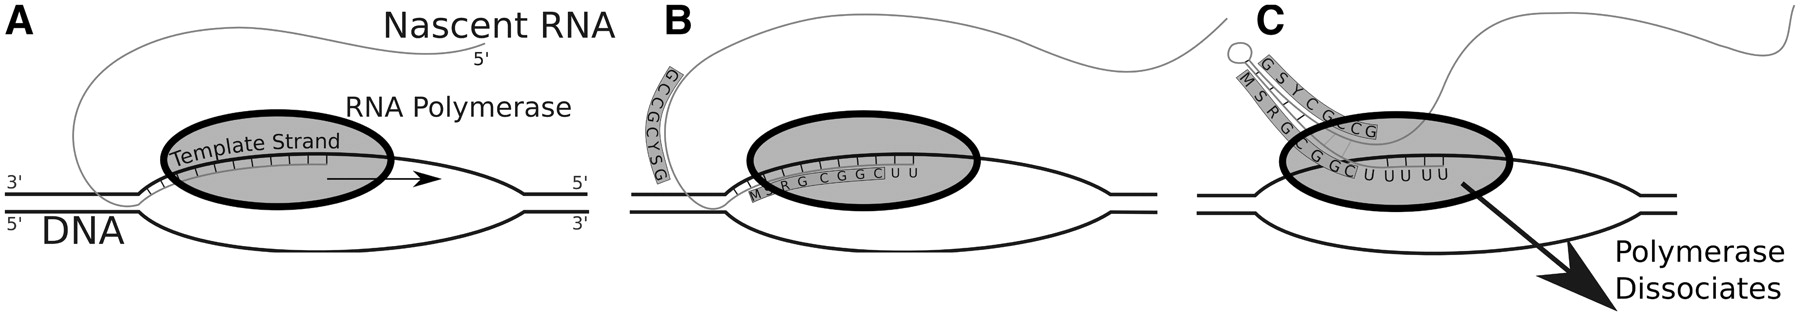
\includegraphics[width=14cm]{rhoindy.jpg}
\caption[Rho-independent termination]{\textbf{Rho-independent termination.} A) The RNA polymerase traverses the DNA template strand from $3^\prime$  to $5^\prime$ , synthesizing the nascent RNA molecule. B) As the polymerase nears a termination site, a G+C-rich terminator stem sequence (boxed) is transcribed. C) Formation of a hairpin structure causes the polymerase to pause, and together with a string of unstable rU-dA bonds causes the polymerase to release from the template. Reproduced from \textcite{Gardner2011a}.
} 
\label{fig:rho}
\end{center}
\end{figure}

The degree to which bacteria rely on intrinsic termination varies widely. A bioinformatic analysis examining the computationally predicted minimum free energy (MFE\nomenclature[Z]{MFE}{Minimum free energy}) of gene termini showed that while some species display an enrichment of strong RNA secondary structures at the $3^\prime$ ends of genes, others do not \parencite{Washio1998}. Mutagenesis studies support this conculsion: while Rho is essential in some genomes with fewer apparent intrinsic terminators (for instance, \textit{Salmonella enterica}, see table \ref{tab:core}), it is dispensable in others that are more heavily dependent on intrinsic termination, such as \textit{Bacillus subtilis} \parencite{Quirk1993}. This suggests competition between the two termination systems, leading to clade-specific skews in RIT utilization \parencite{Carafa1990, Kroger1998, Hoon2005}. The accurate prediction of these elements is critical to understanding the regulation of transcript, particularly in light of the $\ge$3000 completed bacterial genomes currently deposited in EMBL-bank. In addition to their obvious role in helping to define operon structures in genomic sequence \parencite{Salgado2013}, they can also be important indicators of cis-RNA regulation \parencite{Henkin2002, Barrick2007, Naville2010}.

\subsection{Previous approaches to identifying intrinsic terminators}

Two main approaches to detecting RITs have been taken over the years: RNA motif descriptors, both expertly constructed \parencite{Lesnik2001} and automatically generated \parencite{Naville2011}; and thermodynamic models of RNA folding to detect hairpins paired with a heuristic scoring scheme for the poly-T tail region \parencite{Ermolaeva2000, Wan2005, Wan2006, Kingsford2007}. Arguably the most popular of these methods has been TransTermHP \parencite{Kingsford2007}, an example of the second approach.

\begin{figure}[htp]
\begin{center}
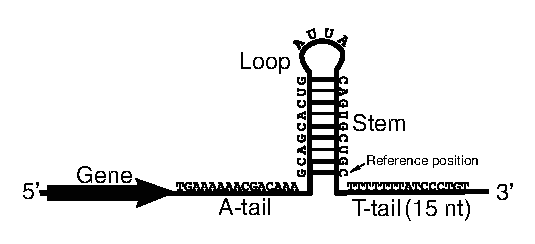
\includegraphics[width=14cm]{transterm}
\caption[TransTermHP motif]{\textbf{TransTermHP motif.} Schematic of the terminator motif that TransTermHP searches for. The terminators consist of a short stem-loop hairpin followed by a thymine-rich region on their $3^\prime$ side. TransTermHP is generally restricted to find terminators where each side of the stem is $\ge$4 nt, the length of the loop is $\ge$3 nt and $\le$13 nt, and the total length of the stem-loop is $\le$59 nt. Reproduced under a Creative Commons Attribution License (CCAL) from \textcite{Kingsford2007}.
} 
\label{fig:transterm}
\end{center}
\end{figure}

The TransTermHP algorithm takes a windowed approach to detecting RITs (figure \ref{fig:transterm}), in common with other thermodynamic approaches. In order to avoid the computational cost of predicting local secondary across the entire genome, TransTermHP first scans overlapping windows of 6 bases for those containing at least 3 T residues. Upon finding such a window, TransTermHP performs a dynamic programming procedure to predict potential hairpin structures, using a simplified version of the Zuker algorithm \parencite{Zuker1981} for {\it in silico} RNA folding parameterized using a set of experimentally validated {\it Escherichia coli} RITs \parencite{Ermolaeva2000}. This is then combined with a heuristic score for the quality of the poly-T tail \parencite{Carafa1990} which rewards T residues occurring closer to the closing base-pairs of the predicted hairpin structure. Candidate RITs are then filtered on stem length, loop length, and total length (see the caption of figure \ref{fig:transterm} for details). Finally, the combined score of surviving candidates is compared to the scores of predicted terminators in random sequence with similar GC content to that of the target genome to provide a measure of prediction quality. Search is apparently also limited to regions surrounding stop codons (\cite{Kingsford2007}; see also the discussion of the beta benchmark below), though the exact boundaries on the search space are not explicitly given in the TransTermHP documentation or publication.

This methodology presents a number of problems. First, while the thermodynamic method used to predict hairpin structures likely places some implicit restrictions on the sequence composition of the hairpin structure, it does not explicitly model conservation of residue composition across terminators. Conservation of residue composition could arise due to convergent evolution of terminator structures under selection for properties that promote strong termination in the host species, or as the results of homology between RITs due to their descent from a common ancestor deposited by transposable elements, as has previously been hypothesized \parencite{Naville2011}. In addition, windowed searching for and heuristic scoring of the poly-T tail is unlikely to accurately capture the true constraints on this feature. We show here that explicitly modelling residue conservation improves detection of RITs. Secondly, the comparison to random sequence with similar GC content is unlikely to be an adequate control: it has been shown that considering dinucleotide content of sequences is critical to determining the significance of their secondary structure \parencite{Workman1999}. Though the method of generating random sequence is not explicitly stated in \textcite{Kingsford2007}, it seems unlikely that it was the product of dinucleotide shuffled sequence or a second-order Markov chain, as would be required to preserve dinucleotide frequencies. In fact TransTermHP does not appear to consider base-stacking effects in its predictions whatsoever. Finally, restricting search to the region around annotated gene termini, or rewarding candidate RITs for being in these regions, is both somewhat artificial and requires accurate gene annotation, which remains a challenge.

\subsection{Covariance models}

\section{Methods}

\section{Results}
\subsection{Alpha benchmark}

\begin{figure}[htp]
\begin{center}
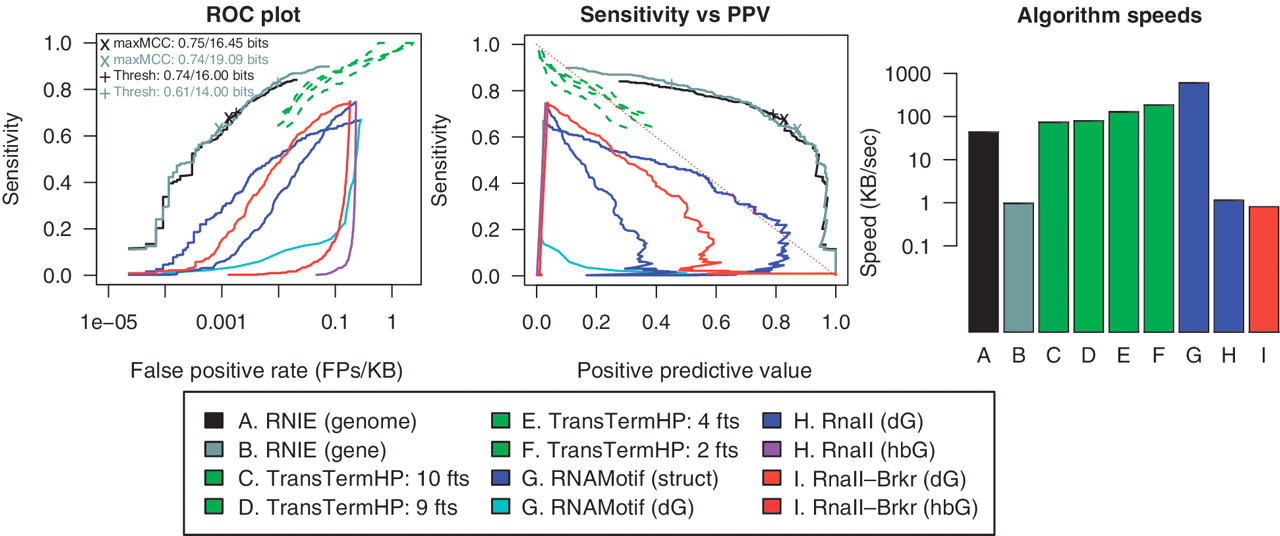
\includegraphics[width=14cm]{alpha.jpg}
\caption[Alpha benchmark]{\textbf{Alpha benchmark.} The accuracy of RNIE compared to existing methods of terminator prediction. The left figure shows a ROC plot for four independent methods. The middle figure compares the sensitivity and PPV for the four methods. The figure on the right shows the speeds for each algorithm in kilobases per second. Reproduced from \textcite{Gardner2011a}.
} 
\label{fig:alpha}
\end{center}
\end{figure}

\subsection{Beta benchmark}

% Table generated by Excel2LaTeX from sheet 'Sheet1'
%
\begingroup
\begin{landscape}
   \tiny
   \noindent
    \begin{longtable}{ l
    				c
				l
				c
				r
				c
				r
				r
				r
				r}
    \caption[Control genomes]{\textbf{Control genomes.} Columns: 1) species name,  2) EMBL-bank accession, 3) phylum, 4) genome size in megabases, 5) number of CDSs annotated in genome, 6) genome G+C content, 7) number of RNIE predictions in genome mode on native sequence, 8) number of RNIE predictions in genome mode on dinucleotide shuffled sequence, 9) number of RNIE predictions in gene mode on native sequence, 10) number of RNIE predictions in gene mode on dinucleotide shuffled sequence.}
    \\
    \toprule
    \textbf{Species} & \textbf{EMBL accession} & \textbf{Phylum} & \textbf{Genome size (MB)} & \textbf{CDSs} & \textbf{G+C content} & \multicolumn{4}{c}{\textbf{Number of predictions}} \\
    & & & & & & \multicolumn{2}{c}{\textbf{Genome}} & \multicolumn{2}{c}{\textbf{Gene}}\\
    & & & & & & \textbf{native} & \textbf{shuffled} & \textbf{native} & \textbf{shuffled}\\
    \midrule
    \textit{Mycobacterium tuberculosis} & AE000516 & Actinobacteria & 4.40 & 4189 & 0.66 & 19 & 0 & 111 & 3\\
    \textit{Streptomyces griseus} & AP009493 & Actinobacteria & 8.55 & 7138 & 0.72 & 72 & 0 & 353 & 2\\
    \textit{Bacteroides thetaiotaomicron} & AE015928 & Bacteroidetes & 6.26 & 4778 & 0.43 & 783 & 2 & 1470 & 44\\
    \textit{Chlamydophila pneumoniae} & AE001363 & Chlamydiae & 1.23 & 1052 & 0.41 & 61 & 3 & 135 & 19\\
    \textit{Prochlorococcus marinus} & AE017126 & Cyanobacteria & 1.75 & 1882 & 0.36 & 81 & 5 & 131 & 22\\
    \textit{Deinococcus radiodurans} & AE000513 & Deinococcus-Thermus & 2.65 & 2579 & 0.67 & 283 & 0 & 506 & 2\\
    \textit{Bacillus subtilis} & AL009126 & Firmicutes & 4.22 & 4245 & 0.44 & 1851 & 4 & 2540 & 54\\
    \textit{Clostridium difficile} & AM180355 & Firmicutes & 4.29 & 3777 & 0.29 & 431 & 8 & 1152 & 58\\
    \textit{Fusobacterium nucleatum} & AE009951 & Fusobacteria & 2.17 & 2067 & 0.27 & 155 & 1 & 457 & 34\\
    \textit{Thermodesulfovibrio yellowstonii} & CP001147 & Nitrospirae & 2.00 & 2033 & 0.34 & 78 & 6 & 176 & 41\\
    \textit{Escherichia coli} & U00096 & Proteobacteria & 4.64 & 4321 & 0.51 & 601 & 6 & 1058 & 35\\
    \textit{Helicobacter pylori} & AE000511 & Proteobacteria & 1.67 & 1566 & 0.39 & 28 & 12 & 128 & 61\\
    \textit{Salmonella enterica} & AE014613 & Proteobacteria & 4.79 & 4323 & 0.52 & 537 & 4 & 980 & 32\\
    \textit{Leptospira interrogans} & AE016823 & Spirochaetes & 4.28 & 3394 & 0.35 & 164 & 18 & 375 & 132\\
    \textit{Ureaplasma parvum} & AF222894 & Tenericutes & 0.75 & 611 & 0.26 & 54 & 0 & 163 & 5\\
    \textit{Fervidobacterium nodosum} & CP000771 & Thermotogae & 1.95 & 1750 & 0.35 & 409 & 3 & 588 & 28\\
    \textit{Methylacidiphilum infernorum} & CP000975 & Verrucomicrobia & 2.29 & 2472 & 0.45 & 50 & 7 & 157 & 52\\
    \bottomrule
    \label{tab:genomes}%
    \end{longtable}%
\end{landscape}%
\endgroup



\begin{figure}[htp]
\begin{center}
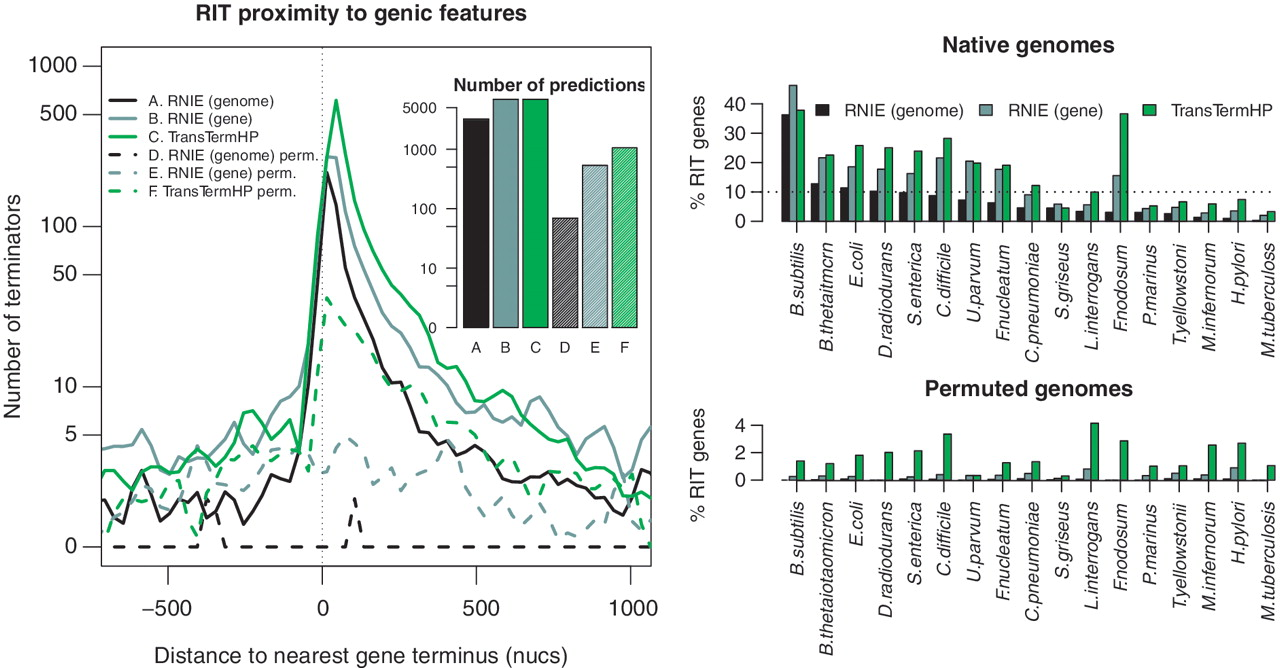
\includegraphics[width=14cm]{beta.jpg}
\caption[Beta benchmark]{\textbf{Beta benchmark.} Ideal terminator predictors will generally produce predictions that are immediately $3^\prime$ to annotated genes on native sequence and no predictions on shuffled controls. For all the test genomes in Table 1 (excluding {\it E. coli} and {\it B. subtilis}), we computed the distance to the nearest $3^\prime$ genic element, including CDSs, ncRNAs and riboswitches. This was done for both native sequences and dinucleotide shuffled control sequences with corresponding gene annotation transferred to the controls. The figure on the left shows the distribution of distances for RNIE genome and gene modes and for the TransTermHP method. Inset is a barplot showing the total number of predictions for each method on native and shuffled genomes. The figures on the right show the percentage of genes that have a predicted RIT in the region $-50$ to $+150$ from an annotated $3^\prime$-end of a CDS or ncRNA across all the genome sequences described in Table 1. The upper panel illustrates the results for the native genomes, while the lower panel illustrates results for the permuted genomes. Reproduced from \textcite{Gardner2011a}.
} 
\label{fig:beta}
\end{center}
\end{figure}

\subsection{A novel termination motif in \textit{Mycobacterium tuberculosis}}

\begin{figure}[htp]
\begin{center}
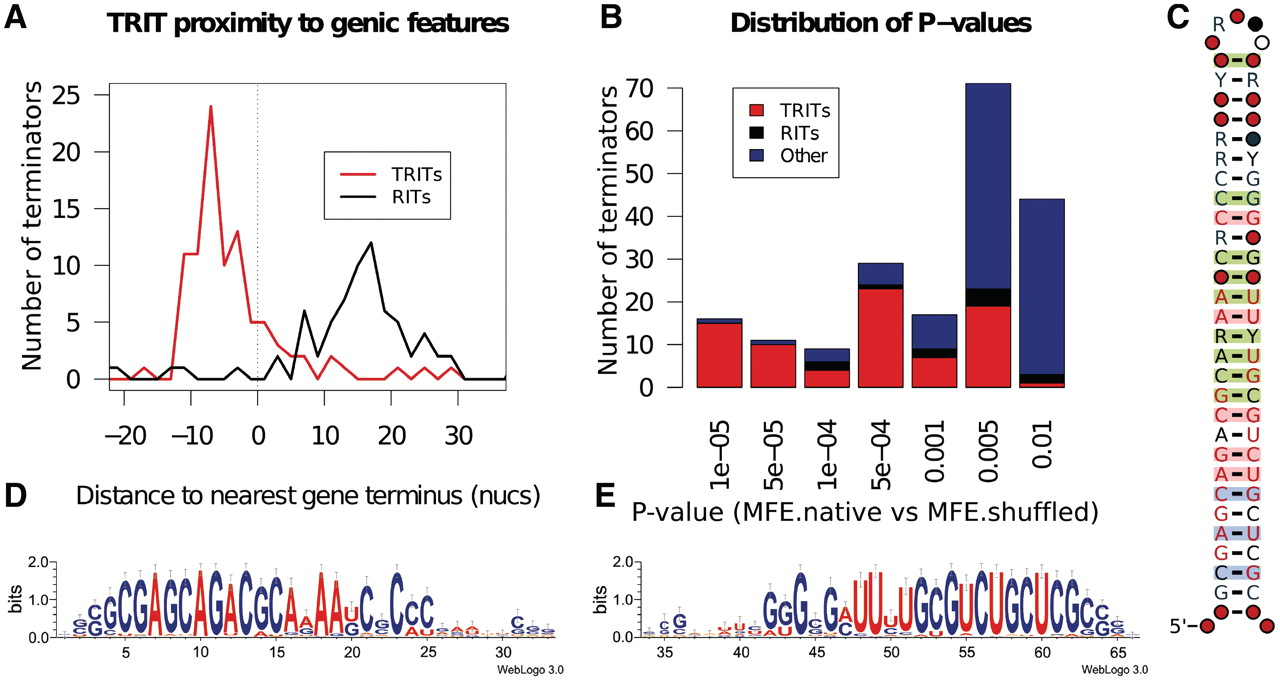
\includegraphics[width=14cm]{myco.jpg}
\caption[Putative mycobacterial transcription termination motif]{\textbf{Putative mycobacterial transcription termination motif.} A) The frequency of TRITs and RITs near the terminal regions of {\it M. tuberculosis} (EMBL accession: AE000516) genic features. B) The distribution of structural stability derived P-values for the most significant {\it M. tuberculosis} terminal regions coloured by TRIT (red), RIT (black) or unclassified (blue). C) The secondary structure and sequence conservation of the TRIT motif as displayed by R2R. (D\&E) Sequence logos generated for the $5^\prime$ D) and $3^\prime$ E) halves of an alignment of the 147 copies of TRIT in the {\it M. tuberculosis} genome. Reproduced from \textcite{Gardner2011a}.
} 
\label{fig:myco}
\end{center}
\end{figure}
